% Options for packages loaded elsewhere
\PassOptionsToPackage{unicode}{hyperref}
\PassOptionsToPackage{hyphens}{url}
%
\documentclass[
]{article}
\usepackage{amsmath,amssymb}
\usepackage{lmodern}
\usepackage{iftex}
\ifPDFTeX
  \usepackage[T1]{fontenc}
  \usepackage[utf8]{inputenc}
  \usepackage{textcomp} % provide euro and other symbols
\else % if luatex or xetex
  \usepackage{unicode-math}
  \defaultfontfeatures{Scale=MatchLowercase}
  \defaultfontfeatures[\rmfamily]{Ligatures=TeX,Scale=1}
\fi
% Use upquote if available, for straight quotes in verbatim environments
\IfFileExists{upquote.sty}{\usepackage{upquote}}{}
\IfFileExists{microtype.sty}{% use microtype if available
  \usepackage[]{microtype}
  \UseMicrotypeSet[protrusion]{basicmath} % disable protrusion for tt fonts
}{}
\makeatletter
\@ifundefined{KOMAClassName}{% if non-KOMA class
  \IfFileExists{parskip.sty}{%
    \usepackage{parskip}
  }{% else
    \setlength{\parindent}{0pt}
    \setlength{\parskip}{6pt plus 2pt minus 1pt}}
}{% if KOMA class
  \KOMAoptions{parskip=half}}
\makeatother
\usepackage{xcolor}
\IfFileExists{xurl.sty}{\usepackage{xurl}}{} % add URL line breaks if available
\IfFileExists{bookmark.sty}{\usepackage{bookmark}}{\usepackage{hyperref}}
\hypersetup{
  pdftitle={Untitled},
  hidelinks,
  pdfcreator={LaTeX via pandoc}}
\urlstyle{same} % disable monospaced font for URLs
\usepackage[margin=1in]{geometry}
\usepackage{color}
\usepackage{fancyvrb}
\newcommand{\VerbBar}{|}
\newcommand{\VERB}{\Verb[commandchars=\\\{\}]}
\DefineVerbatimEnvironment{Highlighting}{Verbatim}{commandchars=\\\{\}}
% Add ',fontsize=\small' for more characters per line
\usepackage{framed}
\definecolor{shadecolor}{RGB}{248,248,248}
\newenvironment{Shaded}{\begin{snugshade}}{\end{snugshade}}
\newcommand{\AlertTok}[1]{\textcolor[rgb]{0.94,0.16,0.16}{#1}}
\newcommand{\AnnotationTok}[1]{\textcolor[rgb]{0.56,0.35,0.01}{\textbf{\textit{#1}}}}
\newcommand{\AttributeTok}[1]{\textcolor[rgb]{0.77,0.63,0.00}{#1}}
\newcommand{\BaseNTok}[1]{\textcolor[rgb]{0.00,0.00,0.81}{#1}}
\newcommand{\BuiltInTok}[1]{#1}
\newcommand{\CharTok}[1]{\textcolor[rgb]{0.31,0.60,0.02}{#1}}
\newcommand{\CommentTok}[1]{\textcolor[rgb]{0.56,0.35,0.01}{\textit{#1}}}
\newcommand{\CommentVarTok}[1]{\textcolor[rgb]{0.56,0.35,0.01}{\textbf{\textit{#1}}}}
\newcommand{\ConstantTok}[1]{\textcolor[rgb]{0.00,0.00,0.00}{#1}}
\newcommand{\ControlFlowTok}[1]{\textcolor[rgb]{0.13,0.29,0.53}{\textbf{#1}}}
\newcommand{\DataTypeTok}[1]{\textcolor[rgb]{0.13,0.29,0.53}{#1}}
\newcommand{\DecValTok}[1]{\textcolor[rgb]{0.00,0.00,0.81}{#1}}
\newcommand{\DocumentationTok}[1]{\textcolor[rgb]{0.56,0.35,0.01}{\textbf{\textit{#1}}}}
\newcommand{\ErrorTok}[1]{\textcolor[rgb]{0.64,0.00,0.00}{\textbf{#1}}}
\newcommand{\ExtensionTok}[1]{#1}
\newcommand{\FloatTok}[1]{\textcolor[rgb]{0.00,0.00,0.81}{#1}}
\newcommand{\FunctionTok}[1]{\textcolor[rgb]{0.00,0.00,0.00}{#1}}
\newcommand{\ImportTok}[1]{#1}
\newcommand{\InformationTok}[1]{\textcolor[rgb]{0.56,0.35,0.01}{\textbf{\textit{#1}}}}
\newcommand{\KeywordTok}[1]{\textcolor[rgb]{0.13,0.29,0.53}{\textbf{#1}}}
\newcommand{\NormalTok}[1]{#1}
\newcommand{\OperatorTok}[1]{\textcolor[rgb]{0.81,0.36,0.00}{\textbf{#1}}}
\newcommand{\OtherTok}[1]{\textcolor[rgb]{0.56,0.35,0.01}{#1}}
\newcommand{\PreprocessorTok}[1]{\textcolor[rgb]{0.56,0.35,0.01}{\textit{#1}}}
\newcommand{\RegionMarkerTok}[1]{#1}
\newcommand{\SpecialCharTok}[1]{\textcolor[rgb]{0.00,0.00,0.00}{#1}}
\newcommand{\SpecialStringTok}[1]{\textcolor[rgb]{0.31,0.60,0.02}{#1}}
\newcommand{\StringTok}[1]{\textcolor[rgb]{0.31,0.60,0.02}{#1}}
\newcommand{\VariableTok}[1]{\textcolor[rgb]{0.00,0.00,0.00}{#1}}
\newcommand{\VerbatimStringTok}[1]{\textcolor[rgb]{0.31,0.60,0.02}{#1}}
\newcommand{\WarningTok}[1]{\textcolor[rgb]{0.56,0.35,0.01}{\textbf{\textit{#1}}}}
\usepackage{longtable,booktabs,array}
\usepackage{calc} % for calculating minipage widths
% Correct order of tables after \paragraph or \subparagraph
\usepackage{etoolbox}
\makeatletter
\patchcmd\longtable{\par}{\if@noskipsec\mbox{}\fi\par}{}{}
\makeatother
% Allow footnotes in longtable head/foot
\IfFileExists{footnotehyper.sty}{\usepackage{footnotehyper}}{\usepackage{footnote}}
\makesavenoteenv{longtable}
\usepackage{graphicx}
\makeatletter
\def\maxwidth{\ifdim\Gin@nat@width>\linewidth\linewidth\else\Gin@nat@width\fi}
\def\maxheight{\ifdim\Gin@nat@height>\textheight\textheight\else\Gin@nat@height\fi}
\makeatother
% Scale images if necessary, so that they will not overflow the page
% margins by default, and it is still possible to overwrite the defaults
% using explicit options in \includegraphics[width, height, ...]{}
\setkeys{Gin}{width=\maxwidth,height=\maxheight,keepaspectratio}
% Set default figure placement to htbp
\makeatletter
\def\fps@figure{htbp}
\makeatother
\setlength{\emergencystretch}{3em} % prevent overfull lines
\providecommand{\tightlist}{%
  \setlength{\itemsep}{0pt}\setlength{\parskip}{0pt}}
\setcounter{secnumdepth}{5}
\usepackage[caption=false]{subfig}
\usepackage{float}
\ifLuaTeX
  \usepackage{selnolig}  % disable illegal ligatures
\fi

\title{Untitled}
\author{}
\date{\vspace{-2.5em}2022-06-11}

\begin{document}
\maketitle

{
\setcounter{tocdepth}{2}
\tableofcontents
}
\begin{verbatim}
## Warning in dir.create("EviewsR_files/"): 'EviewsR_files' already exists
\end{verbatim}

\begin{Shaded}
\begin{Highlighting}[]
\SpecialCharTok{\textgreater{}} \FunctionTok{eviews\_import}\NormalTok{(}\AttributeTok{source\_description =} \StringTok{"EviewsR\_Files/EviewsR\_eviews\_import.csv"}\NormalTok{,}\AttributeTok{frequency =} \StringTok{"m"}\NormalTok{,}\AttributeTok{start\_date =} \StringTok{"1990"}\NormalTok{,}\AttributeTok{save\_path =}\StringTok{\textquotesingle{}EviewsR\_Files\textquotesingle{}}\NormalTok{ )}
\end{Highlighting}
\end{Shaded}

\begin{Shaded}
\begin{Highlighting}[]
\SpecialCharTok{\textgreater{}} \FunctionTok{eviews\_import}\NormalTok{(}\AttributeTok{source\_description =} \StringTok{"EviewsR\_files/EviewsR\_eviews\_import.csv"}\NormalTok{,}\AttributeTok{smpl\_string =} \StringTok{"1990m10 1992m11"}\NormalTok{,}
\SpecialCharTok{+} \AttributeTok{rename\_string =} \StringTok{"x x2"}\NormalTok{)}
\end{Highlighting}
\end{Shaded}

\begin{Shaded}
\begin{Highlighting}[]
\NormalTok{\textgreater{} }\FunctionTok{\textbackslash{}usetikzlibrary}\NormalTok{\{calc\}}
\NormalTok{+ }\FunctionTok{\textbackslash{}usetikzlibrary}\NormalTok{\{positioning\}}
\NormalTok{+ }\FunctionTok{\textbackslash{}usetikzlibrary}\NormalTok{\{arrows\}}
\NormalTok{+   }\KeywordTok{\textbackslash{}begin}\NormalTok{\{}\ExtensionTok{tikzpicture}\NormalTok{\}[}
\NormalTok{+     sharp corners=2pt,}
\NormalTok{+     inner sep=7pt,}
\NormalTok{+     node distance=3cm,}
\NormalTok{+     \textgreater{}=latex]}
\NormalTok{+ }\FunctionTok{\textbackslash{}tikzstyle}\NormalTok{\{my node\}=[draw,minimum height=1cm,minimum width=2cm]}
\NormalTok{+ }\FunctionTok{\textbackslash{}node}\NormalTok{[my node] (A)\{A\};}
\NormalTok{+ }\FunctionTok{\textbackslash{}node}\NormalTok{[my node,right of=A](C)\{C\};}
\NormalTok{+ }\FunctionTok{\textbackslash{}node}\NormalTok{[my node] at (}\SpecialStringTok{$(A)!0.5!(C){-}(0pt,1.5cm)$}\NormalTok{) (B) \{B\};}
\NormalTok{+ }\FunctionTok{\textbackslash{}draw}\NormalTok{[{-}\textgreater{}] (A) {-}{-} (B);}
\NormalTok{+ }\FunctionTok{\textbackslash{}draw}\NormalTok{[{-}\textgreater{}] (A) {-}{-} (C);}
\NormalTok{+ }\FunctionTok{\textbackslash{}draw}\NormalTok{[{-}\textgreater{}] (B) {-}{-} (C);}
\NormalTok{+ }\KeywordTok{\textbackslash{}end}\NormalTok{\{}\ExtensionTok{tikzpicture}\NormalTok{\}}
\end{Highlighting}
\end{Shaded}

\begin{figure}[h]

{\centering 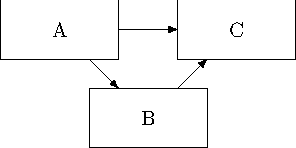
\includegraphics{test_files/figure-latex/ThreeStateDiagram-1} 

}

\caption{Layout of the MSM used in the motivating model}\label{fig:ThreeStateDiagram}
\end{figure}

\end{document}
